\chapter{Multi-Objective Optimization}
\label{ch:multi-objective}

\begin{outcome}
\begin{itemize}
    \item Define multi-objective optimization problems
    \item Discuss solutions in terms of the \emph{Pareto Frontier}
    \item Explore approaches for finding the Pareto Frontier
    \item Use software to solve for or approximate the Pareto Frontier
\end{itemize}
\end{outcome}

\begin{quote}
\itshape You are shopping for a used car. One is \$4{,}000 and twelve years old; another is \$9{,}000 and three years old; a third is \$11{,}000 and eight years old. The third can be dismissed at a glance: the second is cheaper \emph{and} newer. But between the first two, no calculation can declare a winner: it depends on what a year of age is worth to you, and that is a judgment, not an optimization. Multi-objective optimization is the study of exactly this situation: ruling out the options nobody should ever choose, and mapping the trade-offs among the ones that remain.
\end{quote}

\section{Introduction to Multi-Objective Optimization}

Decision makers must often balance competing objectives. Rather than optimizing a single quantity, we seek solutions that trade off different goals, such as cost against quality or efficiency against equity. This leads to the field of \emph{multi-objective optimization} (MOO), a framework for identifying and analyzing such trade-offs.

To illustrate this, consider a simple inventory and production planning problem over a fixed horizon of \(T = 10\) periods. Let \(x_t\) denote the quantity produced in period \(t\), \(s_t\) the inventory carried over after period \(t\), and \(d_t\) the demand to be satisfied during that period. The system begins with \(s_0 = 5\) units of initial inventory. Production costs \(c^p_t\) vary by time, while holding inventory incurs a fixed per-unit cost \(c^h\).

\textbf{The inventory balance constraint} for each period is:
\[
s_t = s_{t-1} + x_t - d_t \quad \text{for all } t = 1,\ldots,T
\]

\textbf{The objective function} (single-objective version) is to minimize total cost:
\[
\min \sum_{t=1}^{T} \left( c^p_t x_t + c^h s_t \right)
\]

However, holding inventory is not just costly; it also introduces risk. Products may be damaged, stolen, or become obsolete. To capture this additional concern, we define a \textbf{risk function} that models the expected loss due to stored inventory:
\[
r(s_t) = c_r \left(1 - e^{-\beta s_t}\right)
\]
where \(c_r\) is the maximum risk cost and \(\beta\) is a sensitivity parameter. This function grows quickly at first, but saturates as inventory increases, reflecting that the marginal risk of storing more units diminishes with protective measures (e.g., insurance, security systems).

\begin{figure}[h]
    \centering
    \altincludegraphics[width=0.65\textwidth]{Figures/risk-plot.pdf}{Plot of the inventory risk function r(s) = c_r(1 - exp(-beta*s)) versus inventory level s: a smooth concave curve rising sharply from zero and saturating toward the maximum risk cost c_r, illustrating that marginal risk diminishes as inventory grows.}
    \caption{Inventory risk cost as a function of inventory level.}
\end{figure}

Now we face a \textbf{multi-objective problem}: we want to minimize both total cost and maximum risk incurred across the planning horizon. These objectives are in tension: reducing risk requires keeping inventory low, which often means producing more frequently at higher cost.

To explore the trade-off, we solve the problem repeatedly with varying upper bounds on inventory (i.e., limiting \(s_t \leq R\)), and for each value compute:
\begin{itemize}
    \item The optimal total cost (production + holding),
    \item The maximum risk experienced across all periods, computed as \( \max_t r(s_t) \).
\end{itemize}

This sweep is the $\varepsilon$-constraint method, which we define later in the chapter (Section~\ref{sec:pareto-frontier}). The parameter values in this example are illustrative; the computational resources at the end of the chapter (Section~\ref{sec:moo-tools}), such as \texttt{pymoo}, make it easy to experiment with instances of your own.

The resulting plot shows the \emph{Pareto frontier} (defined precisely in Section~\ref{sec:pareto-frontier}) of non-dominated solutions, those for which no other solution achieves both a lower cost and lower risk.

\begin{figure}[h]
    \centering
    \altincludegraphics[width=0.7\textwidth]{Figures/pareto-curve.pdf}{Pareto frontier curve for the multi-objective inventory problem, plotting total cost (horizontal axis) against maximum inventory risk (vertical axis). The downward-sloping non-dominated trade-off curve shows that lower risk can only be achieved by accepting higher cost.}
    \caption{Trade-off between total cost and maximum inventory risk.}
\end{figure}

This example illustrates the essence of multi-objective optimization: generating and analyzing a spectrum of solutions that offer different balances between competing goals. In practice, decision makers select among these using domain knowledge, regulatory limits, or stakeholder preferences.

\section{Multi-Objective Optimization and the Pareto Frontier}
\label{sec:pareto-frontier}

We now make these ideas precise. The central concept is the \emph{Pareto Frontier} (or \emph{Pareto Front}), which consists of all solutions for which no objective can be improved without worsening at least one other.

\paragraph{Motivating Example: Furniture Manufacturer}

Consider a high-end furniture manufacturer that builds dining tables and chairs from expensive bocote and rosewood.
The manufacturer receives 960 board-feet (bdft) of bocote and 200 bdft of rosewood per month. Each table requires 80~bdft of bocote and 12~bdft of rosewood; each chair requires 20~bdft of bocote and 10~bdft of rosewood. Let \(x\) denote the number of tables and \(y\) the number of chairs produced. The feasible production set \(P\) is given by:

\[
\begin{aligned}
P = \{(x,y) \in \mathbb{R}^2 :\,& 80x + 20y \le 960,\\
                                   & 12x + 10y \le 200,\\
                                   & x, y \ge 0 \}.
\end{aligned}
\]

\begin{figure}[h]
    \centering
    
    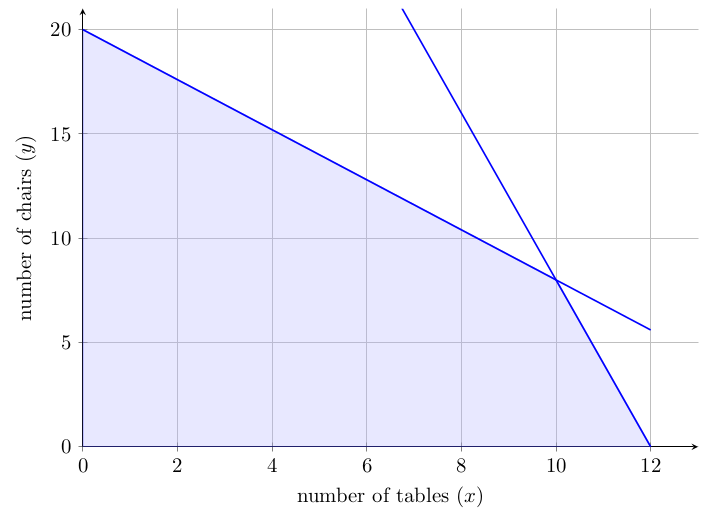
\includegraphics[width=4.71in]{figs/multi-objective-optimization_updated-tikz01.png}
    \caption{Feasible region for the furniture production problem.}
\end{figure}

Suppose each table earns \$8000 and each chair earns \$2000. The goal is to maximize revenue:

\[
\text{Maximize } 8000x + 2000y \quad \text{subject to } (x, y) \in P.
\]

Scaling the objective to \(w = 4x + y\), the feasible region remains the same but is easier to visualize. Solving this LP reveals multiple optimal solutions on the boundary from \((12, 0)\) to \((10, 8)\). These all yield the same profit, but they may differ in other criteria.

Now, suppose a new manager wants to minimize material waste, specifically 10~bdft wasted per table and 2~bdft per chair:

\[
\text{Minimize } 10x + 2y \quad \text{subject to maximum revenue}.
\]

Restricting attention to the profit-optimal frontier and minimizing waste identifies \((10, 8)\) as preferable. This is an example of the \emph{lexicographic method}: optimize a primary objective, then refine solutions with a secondary one.

Alternatively, the manager may be willing to sacrifice some revenue. If they accept at least 70\% of maximum profit, they solve:

\[
\begin{aligned}
\text{Minimize } &\, 10x + 2y \\
\text{subject to } &\, 8000x + 2000y \ge 0.7 \times 96000,\\
&\, (x, y) \in P.
\end{aligned}
\]

\begin{figure}[h]
    \centering
            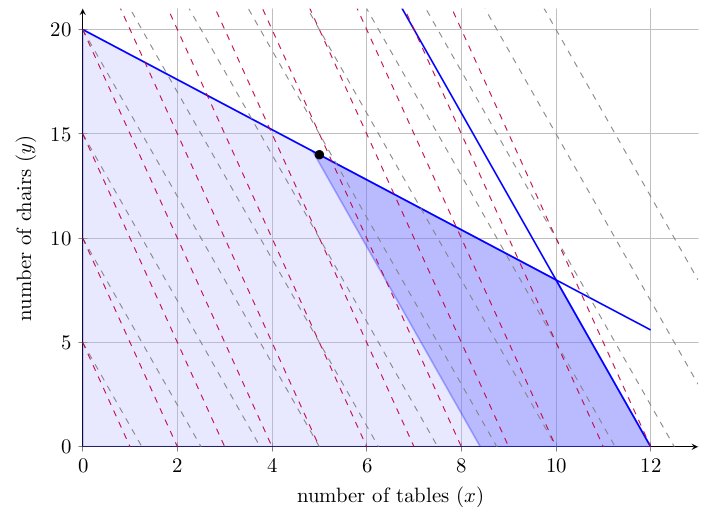
\includegraphics[width=4.71in]{figs/multi-objective-optimization_updated-tikz02.png}
    \caption{Feasible set with revenue constrained to at least 70\% of the maximum.}
\end{figure}

This \emph{$\varepsilon$-constraint} method provides flexibility to explore trade-offs, generating new points on the Pareto frontier.

\paragraph{Pareto Optimality}

Many feasible solutions exist, but only some are \emph{Pareto optimal}. A solution is Pareto optimal if no other feasible solution improves one objective without worsening another.

\begin{definition}{Pareto Optimal}
Given a feasible set \(P\) and objective functions \(f_i: P \to \mathbb{R}\) to \emph{maximize}, a point \(\mathbf{x} \in P\) is \emph{Pareto Optimal} if there is no \(\overline{\mathbf{x}} \in P\) such that:
\[
\begin{aligned}
& f_i(\overline{\mathbf{x}}) > f_i(\mathbf{x}) \text{ for some } i, \\
& f_j(\overline{\mathbf{x}}) \ge f_j(\mathbf{x}) \text{ for all } j \ne i.
\end{aligned}
\]
That is, no objective can be strictly improved without sacrificing performance in at least one other. The \emph{Pareto Frontier} is the set of all such efficient points.
\end{definition}

\begin{figure}[h]
    \centering

            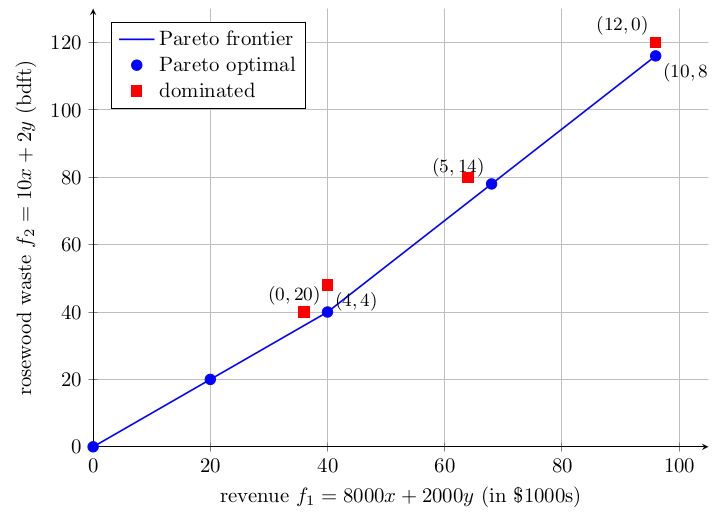
\includegraphics[width=4.79in]{figs/multi-objective-optimization_updated-tikz03.png}
    \caption{The furniture problem in objective space: each point is a production plan $(x,y)$ plotted by its revenue $f_1$ (maximize) and rosewood waste $f_2$ (minimize). The blue points are non-dominated: no feasible plan earns more revenue without creating more waste, and none creates less waste without giving up revenue. The red points are dominated; for example, $(12,0)$ earns the same \$96{,}000 as $(10,8)$ but wastes 120~bdft instead of 116, and $(4,4)$ matches the revenue of $(0,20)$ with more waste. The frontier consists of the plans along $x = 0$ and along the rosewood constraint from $(0,20)$ to $(10,8)$.}
\end{figure}

\paragraph{Summary of Multi-Objective Optimization Methods}

\begin{table}[h]
\centering
\caption{Summary of Multi-Objective Optimization Methods}
\label{tab:moo-methods}
\renewcommand{\arraystretch}{1.3}
\begin{tabular}{|l|p{4.2cm}|p{3.5cm}|p{3.5cm}|}
\hline
\textbf{Method} & \textbf{Key Idea} & \textbf{Pros} & \textbf{Cons} \\
\hline
\textbf{Weighted Sum} & Combine objectives into a single scalar using a weighted sum & Simple and computationally efficient & May miss Pareto-optimal solutions in non-convex regions \\
\hline
\textbf{Lexicographic} & Prioritize objectives in strict order & Matches real-world decision hierarchies & Does not explore trade-offs or the full frontier \\
\hline
\textbf{Epsilon-Constraint} & Optimize one objective, treat others as constraints & Finds non-convex parts of the frontier & Requires repeated solves, hard to set $\varepsilon$ \\
\hline
\textbf{Goal Programming} & Minimize deviation from target values & Useful when goals are known & Sensitive to target and weight choices \\
\hline
\textbf{Elbow (Knee Point)} & Pick the frontier point where trade-offs deteriorate fastest & Yields a single balanced compromise & Requires computing the frontier first; not every frontier has a clear knee \\
\hline
\end{tabular}
\end{table}

\paragraph{Scalarization (Weighted Sum) Method}
The \emph{weighted sum} method transforms a multi-objective optimization problem into a single-objective one by combining the objectives linearly.
For two objectives $f_1(x)$ and $f_2(x)$ (both to be minimized), the scalarized problem takes the form:
\begin{align*}
\min_{x \in X} \quad & w_1 f_1(x) + w_2 f_2(x) \\
\text{s.t.} \quad & x \in X, \quad w_1, w_2 \ge 0, \quad w_1 + w_2 = 1.
\end{align*}
Here, $w_1$ and $w_2$ represent the relative importance of each objective. Varying the weights traces out the \emph{convex} portions of the Pareto frontier: each weight vector corresponds to a supporting hyperplane to the feasible region in objective space.
While simple and computationally efficient, the method \emph{cannot} produce Pareto-optimal points lying in non-convex regions of the frontier. Objectives should be normalized before weighting to ensure that units and scales do not distort the trade-off.

\paragraph{Lexicographic Method}
The \emph{lexicographic} method ranks the objectives in strict order of priority and optimizes them sequentially: first optimize the most important objective, then optimize the second over the set of solutions that are optimal for the first, and so on. This is what the furniture manufacturer did above: maximize revenue first, then minimize rosewood waste among the revenue-optimal plans, which selected $(10,8)$. The method fits settings with a clear hierarchy of goals, but it returns a single solution rather than a picture of the trade-offs.

\paragraph{Goal Programming}
\emph{Goal programming} incorporates explicit target values for each objective, seeking solutions that minimize the deviations from these goals. Let $g_j$ be the desired goal for objective $f_j(x)$. Introduce positive and negative deviation variables $d_j^+$ and $d_j^-$ such that:
\begin{align*}
f_j(x) + d_j^- - d_j^+ = g_j, \quad d_j^+, d_j^- \ge 0.
\end{align*}
A \emph{weighted} goal programming model minimizes a weighted sum of deviations:
\begin{align*}
\min_{x, d^+, d^-} \quad & \sum_{j=1}^m w_j (d_j^+ + d_j^-), \\
\text{s.t.} \quad & x \in X, \; \text{and the above deviation equations hold.}
\end{align*}
The weights $w_j$ reflect the relative penalty for missing each goal. 
In \emph{preemptive} (lexicographic) goal programming, objectives are ranked in priority and optimized sequentially, ensuring higher-priority goals are satisfied as well as possible before addressing lower-priority ones.

\paragraph{Elbow (Knee Point) Method}
When the Pareto frontier is plotted, some decision makers prefer to choose a single compromise point where further improvement in one objective would cause a disproportionately large loss in another. This \emph{elbow} or \emph{knee point} is often found where the curvature of the frontier is largest. 
For discrete Pareto points, a common heuristic is:
\begin{enumerate}
    \item Identify the extreme solutions (best in each objective).
    \item Draw the straight line connecting these extremes in objective space.
    \item Compute the perpendicular distance of each Pareto point to this line.
    \item Select the point with the largest distance as the elbow.
\end{enumerate}
In more formal terms, for a smooth frontier $(f_1(t), f_2(t))$, the knee corresponds to the value of $t$ maximizing the curvature:
\begin{align*}
\kappa(t) = \frac{|f_1'(t) f_2''(t) - f_2'(t) f_1''(t)|}{\left[ (f_1'(t))^2 + (f_2'(t))^2 \right]^{3/2}}.
\end{align*}
Not all Pareto fronts have a clear elbow, and objectives should be normalized to avoid scale bias.
\paragraph{Epsilon-Constraint Method}
The \emph{$\varepsilon$-constraint} method selects one objective as the primary optimization target and converts all other objectives into constraints with adjustable bounds. 
For two objectives $f_1(x)$ and $f_2(x)$ (both to be minimized), one might solve:
\begin{align*}
\min_{x \in X} \quad & f_1(x) \\
\text{s.t.} \quad & f_2(x) \le \varepsilon, \\
& x \in X,
\end{align*}
where $\varepsilon$ is varied across a range of values to generate the Pareto frontier. This method can find both convex and non-convex portions of the frontier, unlike the weighted sum approach. The main practical challenge is choosing meaningful $\varepsilon$ values and step sizes. 
Graphically, this corresponds to sweeping a horizontal (or vertical) constraint across the feasible objective region and optimizing within each slice.
\subsection{Applications of Pareto Frontiers}

Although our furniture example was small, multi-objective optimization arises naturally in many fields.  In each case below, the decision-maker faces competing objectives and must choose a preferred trade-off along the Pareto frontier.

\subsubsection{Portfolio Optimization}
In finance, the classical Markowitz model seeks portfolios that trade off \emph{expected return} against \emph{risk} (variance of return).  Given $n$ assets with expected return vector $\mu \in \R^n$ and covariance matrix $\Sigma \in \R^{n \times n}$, the bi-objective problem is
\[
\max \; \mu^\top w, \qquad \min \; w^\top \Sigma\, w, \qquad \text{subject to} \quad \mathbf{1}^\top w = 1, \; w \geq 0.
\]
The Pareto frontier of this problem is the well-known \emph{efficient frontier}: a curve in the risk--return plane.  Every portfolio on this curve is Pareto optimal; portfolios below it are dominated (higher risk for the same return, or lower return for the same risk).

\subsubsection{Engineering Design}
Mechanical and aerospace engineers routinely face multi-objective trade-offs.  For example, in aircraft wing design the objectives might include minimizing weight (for fuel efficiency), minimizing drag (for speed), and minimizing manufacturing cost, all subject to structural safety constraints.  The Pareto frontier reveals which designs are non-dominated, allowing the engineer to select a final design that best matches operational priorities.  Similar trade-offs arise in automotive design, where ride comfort, fuel economy, and acceleration performance compete.

\subsubsection{Healthcare Staff Scheduling}
Hospitals scheduling nurses and physicians must balance staffing cost against quality-of-care and workload fairness.  Adding staff to a shift reduces patient-to-nurse ratios and overtime fatigue but increases cost; concentrating shifts among fewer workers saves money but hurts fairness and increases burnout risk.  A bi-objective model minimizing total staffing cost and, say, the maximum number of undesirable shifts assigned to any one nurse produces a Pareto frontier of schedules.  Administrators can then see exactly how much each improvement in fairness costs, rather than committing to a single weighting in advance.

\subsubsection{Supply Chain and Sustainability}
Firms increasingly aim to minimize both cost and environmental impact in their supply chains.  A manufacturer might seek to minimize total logistics cost while also minimizing carbon emissions from transportation.  Cheaper shipping routes (e.g., by truck over longer distances) may produce more emissions than costlier alternatives (e.g., rail).  The Pareto frontier shows the achievable trade-offs, helping firms meet sustainability targets at the lowest additional cost.

\section{Computational Tools for Multi-Objective Optimization}
\label{sec:moo-tools}

\begin{resource}
\begin{itemize}
\item \href{https://pymoo.org/}{pymoo: Python Multi-Objective Optimization Framework}
\item \href{https://platemo.com/}{PlatEMO: Platform for Evolutionary Multi-Objective Optimization}
\end{itemize}
\end{resource}

For problems with more than two or three objectives, or with large numbers of decision variables, the exact methods discussed above (weighted sum, $\varepsilon$-constraint) can become computationally expensive. In practice, multi-objective evolutionary algorithms (MOEAs) are widely used to generate high-quality approximations of the Pareto frontier.

Several well-known algorithms are available for this purpose:
\begin{description}
\item[NSGA-II] (Non-dominated Sorting Genetic Algorithm II) is one of the most widely used MOEAs. It maintains a population of candidate solutions and uses non-dominated sorting together with a crowding distance metric to preserve diversity along the Pareto front. NSGA-II is effective for problems with two or three objectives.
\item[NSGA-III] extends NSGA-II to handle many-objective problems (four or more objectives) by using reference directions instead of crowding distance to maintain a well-distributed set of solutions across the Pareto frontier.
\item[MOEA/D] (Multi-Objective Evolutionary Algorithm based on Decomposition) decomposes the multi-objective problem into a collection of single-objective subproblems using weight vectors, solving them simultaneously. This approach is particularly effective when the Pareto frontier has a regular structure.
\end{description}

The Python library \texttt{pymoo} provides implementations of these algorithms and many others, along with built-in test problems, performance metrics, and visualization tools for Pareto fronts. It offers a convenient way to experiment with multi-objective optimization without implementing algorithms from scratch.

For small problems like the furniture example, the $\varepsilon$-constraint method needs nothing more than an ordinary LP solver. The following PuLP script maximizes revenue while sweeping the bound on rosewood waste, recovering points on the Pareto frontier:

\begin{lstlisting}[language=Python]
import pulp

for eps in [40, 60, 80, 100, 116]:
    prob = pulp.LpProblem("furniture", pulp.LpMaximize)
    x = pulp.LpVariable("tables", lowBound=0)
    y = pulp.LpVariable("chairs", lowBound=0)
    prob += 8000*x + 2000*y            # revenue (primary objective)
    prob += 80*x + 20*y <= 960         # bocote
    prob += 12*x + 10*y <= 200         # rosewood
    prob += 10*x + 2*y <= eps          # waste <= epsilon
    prob.solve(pulp.PULP_CBC_CMD(msg=0))
    print(f"eps={eps}: x={x.value():.2f}, y={y.value():.2f}, "
          f"revenue={pulp.value(prob.objective):.0f}")
\end{lstlisting}

Sweeping $\varepsilon$ from 40 to 116 traces the frontier from the plan $(0,20)$ with revenue \$40{,}000 up to $(10,8)$ with revenue \$96{,}000, passing through fractional plans such as $x \approx 5.26$, $y \approx 13.68$ with revenue \$69{,}474 at $\varepsilon = 80$.

\section{Exercises}

\exgroup{Warm-ups}

\begin{ex}{Defining Pareto Optimality}{}
\stars{1}\label{ex:pareto-def}
Define \emph{Pareto optimality} for a minimization multi-objective problem with two objectives.
\exrefs{Section~\ref{sec:pareto-frontier}}
\end{ex}

\begin{ex}{Spotting Dominated Designs}{}
\stars{1}\label{ex:moo-dominance}
Five supplier contracts are scored on two objectives, both to be minimized: $f_1$ (cost, in \$1000s) and $f_2$ (delivery time, in days).

\begin{center}
\begin{tabular}{c|ccccc}
Contract & G & H & I & J & K \\\hline
$f_1$    & 2 & 4 & 5 & 7 & 6 \\
$f_2$    & 9 & 7 & 8 & 3 & 5 \\
\end{tabular}
\end{center}

\begin{enumerate}
\item Which contracts are dominated, and by which contract?
\item List the Pareto frontier in order of increasing $f_1$.
\item True or false: a contract that is the unique minimizer of $f_1$ can never be dominated. Explain.
\end{enumerate}
\exrefs{Section~\ref{sec:pareto-frontier}, Exercise~\ref{ex:pareto-table}}
\end{ex}

\begin{ex}{Computing Weighted-Sum Scores}{}
\stars{1}\label{ex:moo-weighted-scores}
Using the contract table from Exercise~\ref{ex:moo-dominance}, form the weighted score $S = w_1 f_1 + w_2 f_2$ (both objectives minimized, so the lowest score wins).
\begin{enumerate}
\item For $(w_1, w_2) = (0.6, 0.4)$, compute all five scores and identify the winning contract.
\item Repeat for $(w_1, w_2) = (0.2, 0.8)$. Why does the winner change?
\item Contract I is dominated by contract H. Show that for every choice of weights $w_1, w_2 > 0$, contract I scores strictly worse than H, so a dominated point can never win a weighted sum with positive weights.
\end{enumerate}
\exrefs{Section~\ref{sec:pareto-frontier}}
\end{ex}

\exgroup{Core problems}

\begin{ex}{Pareto Frontier, Weighted Sum, and $\varepsilon$-Constraint}{}
\stars{2}\label{ex:pareto-table}
Consider the following feasible set of designs with two objectives to minimize: $f_1$ (cost) and $f_2$ (emissions).
The table lists six \emph{candidates} from a design study; some may be dominated among this set.

\begin{center}
\begin{tabular}{c|cccccc}
Design & A & B & C & D & E & F \\\hline
$f_1$  & 6 & 4 & 7 & 3 & 5 & 10 \\
$f_2$  & 5 & 8 & 4 & 6 & 6 & 3 \\
\end{tabular}
\end{center}

\begin{enumerate}
\item Identify all \textbf{Pareto optimal} designs from $\{A,\ldots,F\}$ and list the Pareto frontier.
\vspace{2cm}

\item Suppose we use a \emph{weighted-sum} with weights $(\alpha,1-\alpha)$, $\alpha\in[0,1]$. Which designs can be obtained as optimal for some $\alpha$? Briefly justify.

\vspace{2cm}

\item Using the $\varepsilon$-constraint method minimizing $f_1$ subject to $f_2\le \varepsilon$, give a value of $\varepsilon$ that attains a design on the frontier \emph{that cannot be obtained} by any weighted sum (if any), or explain why all frontier points are reachable by weighted sums.

\vspace{2cm}

\item Sketch (by hand) the points in the $(f_1,f_2)$ plane, indicate dominated points, and draw the Pareto frontier with arrows showing the direction of improvement.

\vspace{6cm}
\end{enumerate}
\exrefs{Section~\ref{sec:pareto-frontier}, Table~\ref{tab:moo-methods}}
\end{ex}

\begin{ex}{Weighted Sum Method}{}
\stars{2}\label{ex:weighted-sum-projects}
A city planner is evaluating three road improvement projects. Each project has a cost (to minimize) and an accessibility score (to maximize):

\begin{center}
\begin{tabular}{c|c|c}
\textbf{Project} & \textbf{Cost (\$M)} & \textbf{Accessibility Score} \\
\hline
P1 & 2 & 7 \\
P2 & 5 & 9 \\
P3 & 3 & 6 \\
\end{tabular}
\end{center}

We reformulate as a minimization problem with objectives $f_1 = \text{cost}$ and $f_2 = -\text{accessibility}$ (so both are minimized).

\begin{enumerate}
\item Which projects are Pareto optimal? Justify your answer.
\item Using the weighted-sum method with weights $w_1 = 0.5$ for cost and $w_2 = 0.5$ for negative accessibility, which project is selected?
\item Is there a set of weights that would select project P3? Explain.
\end{enumerate}
\exrefs{Section~\ref{sec:pareto-frontier}}
\end{ex}

\begin{ex}{Epsilon-Constraint Method}{}
\stars{2}\label{ex:eps-constraint-lp}
Consider a bi-objective linear program:
\[
\min \; (f_1(\mathbf{x}), \; f_2(\mathbf{x})) = (x_1 + 2x_2, \; 3x_1 + x_2)
\]
subject to $x_1 + x_2 \geq 4$, $x_1 \leq 5$, $x_2 \leq 5$, and $x_1, x_2 \geq 0$.

\begin{enumerate}
\item Apply the $\varepsilon$-constraint method: minimize $f_1$ subject to $f_2 \leq \varepsilon$. Write out the resulting single-objective LP.
\item Find the optimal solution for $\varepsilon = 10$ and for $\varepsilon = 6$. Are both solutions Pareto optimal?
\item Describe what happens as $\varepsilon$ decreases from a large value toward $f_2^*$ (the minimum of $f_2$ alone).
\end{enumerate}
\exrefs{Section~\ref{sec:pareto-frontier}, Section~\ref{sec:moo-tools}}
\end{ex}

\begin{ex}{Epsilon-Constraint by Hand}{}
\stars{2}\label{ex:eps-triangle}
Consider two objectives to \emph{maximize}, $f_1 = 3x_1 + x_2$ and $f_2 = x_1 + 3x_2$, over the triangle
\[
X = \{(x_1, x_2) \geq 0 : x_1 + x_2 \leq 6\}.
\]
\begin{enumerate}
\item Evaluate both objectives at the three vertices of $X$. Which vertex maximizes $f_1$ alone? Which maximizes $f_2$ alone?
\item Apply the $\varepsilon$-constraint method: maximize $f_1$ subject to $f_2 \geq \varepsilon$ and $x \in X$, for each $\varepsilon \in \{6, 10, 14, 18\}$. Solve each LP by hand (graphically, or by checking the vertices of the sliced region) and tabulate $(x_1, x_2, f_1, f_2)$.
\item Which part of the boundary of $X$ is the Pareto frontier in decision space? What is the trade-off rate between $f_1$ and $f_2$ along it?
\item What happens if $\varepsilon > 18$?
\end{enumerate}
\exrefs{Section~\ref{sec:pareto-frontier}, Section~\ref{sec:moo-tools}}
\end{ex}

\begin{ex}{Trade-Off Analysis}{}
\stars{2}\label{ex:tradeoff-analysis}
A manufacturing firm faces two conflicting objectives: minimizing production cost ($f_1$) and minimizing environmental emissions ($f_2$). After solving a series of weighted-sum problems, the following Pareto optimal solutions are found:

\begin{center}
\begin{tabular}{c|c|c}
\textbf{Solution} & $f_1$ \textbf{(Cost, \$1000s)} & $f_2$ \textbf{(Emissions, tons)} \\
\hline
S1 & 40 & 20 \\
S2 & 45 & 14 \\
S3 & 55 & 10 \\
S4 & 70 & 8 \\
\end{tabular}
\end{center}

\begin{enumerate}
\item Plot these points in the objective space. Draw the Pareto frontier.
\item Compute the marginal rate of substitution (trade-off ratio) between each consecutive pair of solutions. Which jump in cost gives the largest reduction in emissions per dollar?
\item If the firm is willing to spend at most \$50{,}000, which Pareto optimal solution should it choose?
\end{enumerate}
\exrefs{Section~\ref{sec:pareto-frontier}}
\end{ex}

\exgroup{Concepts and connections}

\begin{ex}{What Weighted Sums Cannot See}{}
\stars{2}\label{ex:nonconvex-weights}
A design study produces exactly three Pareto optimal outcomes in objective space, both objectives minimized:
\[
P = (0, 4), \qquad Q = (3, 3), \qquad R = (4, 0).
\]
\begin{enumerate}
\item Verify that no one of these points dominates another.
\item For weights $(\alpha, 1-\alpha)$ with $\alpha \in [0,1]$, write the weighted score of each point as a function of $\alpha$ and show that $\min\{4\alpha,\, 4 - 4\alpha\} \leq 2 < 3$ for every $\alpha$. Conclude that $Q$ is never a weighted-sum optimum, not even tied.
\item Explain the result geometrically: which points lie on the lower convex hull of $\{P, Q, R\}$, and why does every weighted sum correspond to a supporting line of that hull? Relate your answer to the ``Cons'' entry for the weighted-sum method in Table~\ref{tab:moo-methods}.
\item Name a method from Table~\ref{tab:moo-methods} that does recover $Q$, and give a specific parameter value for it that works.
\end{enumerate}
\exrefs{Section~\ref{sec:pareto-frontier}, Table~\ref{tab:moo-methods}}
\end{ex}

\begin{ex}{Lexicographic versus Weighted Sum}{}
\stars{2}\label{ex:lex-vs-weighted}
In the furniture example of Section~\ref{sec:pareto-frontier}, the lexicographic method (maximize revenue first, then minimize waste among revenue-optimal plans) selects $(10, 8)$.
\begin{enumerate}
\item A weighted sum with all weight on revenue ($\alpha = 1$) maximizes $8000x + 2000y$ alone. Which plans are optimal then, and why does this not reproduce the lexicographic answer?
\item Argue that any weight $\alpha < 1$ close enough to $1$ selects exactly $(10, 8)$: the small weight on waste acts as a tie-breaker among revenue-optimal plans while being too small to justify giving up revenue. (Exercise~\ref{ex:furniture-weights} computes the exact threshold.)
\item When do the two methods agree in general? Explain why for a linear program with finitely many vertices there is always a sufficiently extreme weight that reproduces the lexicographic solution, and describe informally what can go wrong if the weight on the secondary objective is not small enough.
\end{enumerate}
\exrefs{Section~\ref{sec:pareto-frontier}, Table~\ref{tab:moo-methods}}
\end{ex}

\exgroup{Challenge problems}

\begin{ex}{Weights That Select Each Vertex}{}
\stars{3}\label{ex:furniture-weights}
Return to the furniture example of Section~\ref{sec:pareto-frontier}. Measure revenue in thousands of dollars, so the objectives are $f_1 = 8x + 2y$ (maximize) and $f_2 = 10x + 2y$ (minimize, waste in bdft). The weighted-sum method solves
\[
\max_{(x,y) \in P} \; \alpha f_1(x,y) - (1-\alpha) f_2(x,y), \qquad \alpha \in [0,1].
\]
\begin{enumerate}
\item The optimum is always attained at a vertex of $P$: $(0,0)$, $(0,20)$, $(10,8)$, or $(12,0)$. Write the weighted objective value of each vertex as a linear function of $\alpha$.
\item For each Pareto optimal vertex, find the exact interval of $\alpha$ for which it is optimal, and give the breakpoint values of $\alpha$.
\item What is optimal exactly at each breakpoint, and at $\alpha = 1$? Explain why the dominated vertex $(12,0)$ shows up at $\alpha = 1$ and what this says about using zero weights.
\item Repeat part (2) with revenue in raw dollars ($f_1 = 8000x + 2000y$). Where are the breakpoints now? What does this tell you about normalizing objectives before choosing weights?
\end{enumerate}
\exrefs{Section~\ref{sec:pareto-frontier}, Table~\ref{tab:moo-methods}}
\end{ex}

\subsubsection*{Selected Solutions}

\begin{solution}(Exercise~\ref{ex:pareto-def})
For a problem minimizing $f_1$ and $f_2$ over a feasible set $P$, a point $\mathbf{x} \in P$ is \emph{Pareto optimal} if there is no $\overline{\mathbf{x}} \in P$ with $f_i(\overline{\mathbf{x}}) \leq f_i(\mathbf{x})$ for both $i = 1, 2$ and $f_i(\overline{\mathbf{x}}) < f_i(\mathbf{x})$ for at least one $i$.  In words: no other feasible point is at least as good in both objectives and strictly better in one.
\end{solution}

\begin{solution}(Exercise~\ref{ex:pareto-table})
(1) Compare pairs for domination (both objectives minimized).  $D = (3,6)$ dominates $B = (4,8)$.  $E = (5,6)$ is dominated by $D$ ($3 \leq 5$, $6 \leq 6$).  $A = (6,5)$ is not dominated.  $C = (7,4)$ is not dominated.  $F = (10,3)$ is not dominated.  The Pareto frontier is $\{D, A, C, F\}$ with objective vectors $(3,6), (6,5), (7,4), (10,3)$.

(2) A design is a weighted-sum optimum for some $\alpha$ exactly when it lies on the lower-left convex hull of the frontier points.  Plotting $(3,6), (6,5), (7,4), (10,3)$, the lower convex hull is formed by $D$, $C$, and $F$, while $A$ lies above it: $D$ (best $f_1$) and $F$ (best $f_2$) are always obtainable, and $C$ lies on the hull between them, but $A$ sits above the segment from $D$ to $C$ (slope check: from $D$ to $C$, $\Delta = (4, -2)$; $A$ at $(6,5)$ vs.\ the segment value $6 - \tfrac{2}{4}(6-3) = 4.5 < 5$), so $A$ cannot be obtained by any weighted sum.

(3) Choose $\varepsilon = 5$: minimizing $f_1$ subject to $f_2 \leq 5$ selects $A = (6,5)$, the frontier point unreachable by weighted sums.
\end{solution}

\begin{solution}(Exercise~\ref{ex:eps-triangle})
(1) At $(0,0)$: $(f_1, f_2) = (0,0)$. At $(6,0)$: $(18, 6)$. At $(0,6)$: $(6, 18)$. So $(6,0)$ maximizes $f_1$ alone and $(0,6)$ maximizes $f_2$ alone.

(2) For $\varepsilon > 6$ the constraint $x_1 + 3x_2 \geq \varepsilon$ is binding at the optimum, and the solution lies where it meets the edge $x_1 + x_2 = 6$: solving the two equations gives $x_2 = (\varepsilon - 6)/2$, $x_1 = (18 - \varepsilon)/2$.
\begin{center}
\begin{tabular}{c|cccc}
$\varepsilon$ & $x_1$ & $x_2$ & $f_1$ & $f_2$ \\\hline
6  & 6 & 0 & 18 & 6 \\
10 & 4 & 2 & 14 & 10 \\
14 & 2 & 4 & 10 & 14 \\
18 & 0 & 6 & 6  & 18 \\
\end{tabular}
\end{center}

(3) Each solution has $f_2 = \varepsilon$ exactly and the largest possible $f_1$ given that, so each is Pareto optimal. The frontier is the edge $x_1 + x_2 = 6$ from $(6,0)$ to $(0,6)$: parametrizing by $x_2 = t$ gives $f_1 = 18 - 2t$ and $f_2 = 6 + 2t$, a one-for-one trade-off between the objectives.

(4) The maximum of $f_2$ over $X$ is $18$, so for $\varepsilon > 18$ the constrained LP is infeasible; the sweep should stop there.
\end{solution}

\begin{solution}(Exercise~\ref{ex:furniture-weights})
(1) The weighted objective $\alpha(8x + 2y) - (1-\alpha)(10x + 2y)$ at each vertex:
\[
(0,0): 0, \qquad
(0,20): 80\alpha - 40, \qquad
(10,8): 212\alpha - 116, \qquad
(12,0): 216\alpha - 120.
\]

(2) The optimal value is the upper envelope of these four linear functions of $\alpha$. Comparing pairs: $(0,20)$ beats $(0,0)$ iff $80\alpha - 40 \geq 0$, i.e., $\alpha \geq \tfrac12$; $(10,8)$ beats $(0,20)$ iff $212\alpha - 116 \geq 80\alpha - 40$, i.e., $132\alpha \geq 76$, i.e., $\alpha \geq \tfrac{19}{33} \approx 0.576$; and $(10,8)$ beats $(12,0)$ iff $4 \geq 4\alpha$, which holds for all $\alpha \leq 1$. Hence
\[
(0,0) \text{ optimal for } \alpha \in [0, \tfrac12], \qquad
(0,20) \text{ for } \alpha \in [\tfrac12, \tfrac{19}{33}], \qquad
(10,8) \text{ for } \alpha \in [\tfrac{19}{33}, 1].
\]
A numerical sweep confirms the switch: $\alpha = 0.5757$ returns $(0,20)$ and $\alpha = 0.5758$ returns $(10,8)$.

(3) At $\alpha = \tfrac12$ the entire edge $x = 0$ is optimal (every plan $(0,y)$ scores $0$ there); at $\alpha = \tfrac{19}{33}$ the whole rosewood edge from $(0,20)$ to $(10,8)$ is optimal. At $\alpha = 1$ waste is ignored, so all revenue-optimal plans, the edge from $(10,8)$ to $(12,0)$, are optimal, including the dominated plan $(12,0)$. A weighted sum with a zero weight can return points that are not Pareto optimal; any positive weight on waste breaks the tie in favor of $(10,8)$.

(4) With $f_1 = 8000x + 2000y$, the same comparisons give breakpoints $\alpha = \tfrac{1}{1001} \approx 0.001$ and $\alpha = \tfrac{19}{14019} \approx 0.00136$: virtually every weight selects $(10,8)$. When objectives live on wildly different scales, the weights lose their intended meaning, which is why objectives should be normalized before weighting (Section~\ref{sec:pareto-frontier}).
\end{solution}
